\documentclass[11pt]{article}\usepackage[]{graphicx}\usepackage[]{color}
%% maxwidth is the original width if it is less than linewidth
%% otherwise use linewidth (to make sure the graphics do not exceed the margin)
\makeatletter
\def\maxwidth{ %
  \ifdim\Gin@nat@width>\linewidth
    \linewidth
  \else
    \Gin@nat@width
  \fi
}
\makeatother

\definecolor{fgcolor}{rgb}{0.345, 0.345, 0.345}
\newcommand{\hlnum}[1]{\textcolor[rgb]{0.686,0.059,0.569}{#1}}%
\newcommand{\hlstr}[1]{\textcolor[rgb]{0.192,0.494,0.8}{#1}}%
\newcommand{\hlcom}[1]{\textcolor[rgb]{0.678,0.584,0.686}{\textit{#1}}}%
\newcommand{\hlopt}[1]{\textcolor[rgb]{0,0,0}{#1}}%
\newcommand{\hlstd}[1]{\textcolor[rgb]{0.345,0.345,0.345}{#1}}%
\newcommand{\hlkwa}[1]{\textcolor[rgb]{0.161,0.373,0.58}{\textbf{#1}}}%
\newcommand{\hlkwb}[1]{\textcolor[rgb]{0.69,0.353,0.396}{#1}}%
\newcommand{\hlkwc}[1]{\textcolor[rgb]{0.333,0.667,0.333}{#1}}%
\newcommand{\hlkwd}[1]{\textcolor[rgb]{0.737,0.353,0.396}{\textbf{#1}}}%
\let\hlipl\hlkwb

\usepackage{framed}
\makeatletter
\newenvironment{kframe}{%
 \def\at@end@of@kframe{}%
 \ifinner\ifhmode%
  \def\at@end@of@kframe{\end{minipage}}%
  \begin{minipage}{\columnwidth}%
 \fi\fi%
 \def\FrameCommand##1{\hskip\@totalleftmargin \hskip-\fboxsep
 \colorbox{shadecolor}{##1}\hskip-\fboxsep
     % There is no \\@totalrightmargin, so:
     \hskip-\linewidth \hskip-\@totalleftmargin \hskip\columnwidth}%
 \MakeFramed {\advance\hsize-\width
   \@totalleftmargin\z@ \linewidth\hsize
   \@setminipage}}%
 {\par\unskip\endMakeFramed%
 \at@end@of@kframe}
\makeatother

\definecolor{shadecolor}{rgb}{.97, .97, .97}
\definecolor{messagecolor}{rgb}{0, 0, 0}
\definecolor{warningcolor}{rgb}{1, 0, 1}
\definecolor{errorcolor}{rgb}{1, 0, 0}
\newenvironment{knitrout}{}{} % an empty environment to be redefined in TeX

\usepackage{alltt}
\usepackage[sc]{mathpazo} %Like Palatino with extensive math support
\usepackage{fullpage}
\usepackage{gensymb}
\usepackage{multirow}
\usepackage{booktabs}
\usepackage{amsmath}
\usepackage[authoryear,sectionbib,sort]{natbib}
\linespread{1.7}
\usepackage[utf8]{inputenc}
\usepackage{lineno}
\usepackage{titlesec}
\titleformat{\section}[block]{\Large\bfseries\filcenter}{\thesection}{1em}{}
\titleformat{\subsection}[block]{\Large\itshape\filcenter}{\thesubsection}{1em}{}
\titleformat{\subsubsection}[block]{\large\itshape}{\thesubsubsection}{1em}{}
\titleformat{\paragraph}[runin]{\itshape}{\theparagraph}{1em}{}[. ]\renewcommand{\refname}{Literature Cited}


\title{Thermal performance of fish is explained by an interplay between physiology, behaviour, and ecology}


% \author{Philipp Neubauer^{1,\ast}$ \\ 
%         Ken H. Andersen$^{2,\dag}$}


\date{}
\IfFileExists{upquote.sty}{\usepackage{upquote}}{}
\begin{document}

\maketitle

% \noindent{} 1. Dragonfly Data Science, PO Box 27535, Wellington 6141, New Zealand;
% 
% \noindent{} 2. Centre for Ocean Life, National Institute of Aquatic Resources, Technical University of Denmark, 7 Kemitorvet B-202, 2800 Kongens Lyngby, Denmark;

\bigskip

\textit{Manuscript elements}: Figure~1, figure~2, table~1, online appendices~A and B (including figure~A1 and figure~A2). Figure~2 is to print in color.

\bigskip

\textit{Keywords}: thermal performance, OCLTT, metabolic rate, climate change

\bigskip

\textit{Manuscript type}: Article.

\bigskip

\noindent{\footnotesize Prepared using the suggested \LaTeX{} template for \textit{Am.\ Nat.}}

\linenumbers{}
\modulolinenumbers[3]

\newpage{}

\section*{Abstract}

Increasing temperatures under climate change are thought to affect individual physiology of fish and other ectotherms through increases in metabolic demands, leading to changes in species performance with concomitant effects on species ecology. Although intuitively appealing, the driving mechanism behind thermal performance is contested: thermal performance (e.g., growth) appears correlated with metabolic scope (i.e., oxygen availability for activity) for a number of species, but a substantial number of datasets do not support oxygen limitation of long-term performance. Whether or not oxygen limitations via the metabolic scope, or a lack thereof, have major ecological consequences remains a highly contested question. Here, we propose a general size and trait-based model of energy and oxygen budgets to determine the relative influence of metabolic rates, oxygen limitation, and environmental conditions on ecotherm performance. We show that oxygen limitation is not necessary to explain performance variation with temperature. Oxygen can drastically limit performance and fitness, especially at temperature extremes, but changes in thermal performance are primarily driven by the interplay between changing metabolic rates and species ecology. Furthermore, our model reveals that fitness trends with temperature can oppose trends in growth, suggesting a potential explanation for the paradox that species often occur at lower temperatures than their growth-optimum. Our model provides a mechanistic underpinning that can provide general and realistic predictions about temperature impacts on the performance of fish and other ectotherms, and act as a null model for contrasting temperature impacts on species with different metabolic and ecological traits.

\newpage

\section*{Introduction}

Temperature, through its effects on individual physiology, is a dominant driver of species ecology and bio-geography (\cite{deutsch_climate_2015,pinsky_marine_2013}). As a consequence, current and predicted temperature increases under climate change will act as a strong agent of change in many ecosystems (\cite{deutsch_climate_2015, stuart-smith_thermal_2015, parmesan_globally_2003, walther_ecological_2002}). However, the nature of these changes can be difficult to predict as temperature effects scale from individuals to species and ecosystems. Through this cascade of scales, incorrect or approximate model assumptions at the individual scale can have disproportionate effects on ecosystem level outcomes (\cite{brander_overconfidence_2013, lefevre_models_2017}). In marine fish, for example, recent predictions of decreasing organism size, and resulting decreases in the size of fisheries catches (\cite{cheung_shrinking_2013}), have been criticized as overly simplistic and not in line with physiological constraints (\cite{brander_overconfidence_2013, lefevre_models_2017,jutfelt_oxygen-and_2018}).

Although there are conceptual and model frameworks to explain aspects of thermal performance and ecological responses to temperature (\cite{fry_effects_1947,brown_toward_2004,pauly_sound_2017,portner_oxygen-and_2010}), many of these remain controversial as they appear limited in their generality or predictive capacity (\cite{lefevre_models_2017,jutfelt_oxygen-and_2018}). To our knowledge, no general theoretical framework exists to quantitatively explain and predict changes in  ecological rates, such as observed change in growth and asymptotic size \cite[e.g., the temerature-size rule in ectotherms;][]{angilletta_temperature_2004,atkinson_temperature_1994}), or attack rates (\cite{englund_temperature_2011,rall_universal_2012}) with temperature, from fundamental physiological processes. Instead, and as advocated by the metabolic theory of ecology (\cite{brown_toward_2004}), ecological theory often treats ecological rates as being directly temperature dependent, without a direct link to the underlying physiological drivers (\cite[e.g., ][]{angilletta_temperature_2004,vucic-pestic_warming_2011, guiet_effects_2016}). 

A phenomenological description that assumes a general ecological temperature response often fails to explain heterogeneity in ecological responses (\cite{angilletta_temperature_2004,rall_universal_2012}). Although ecological rates seem to follow some general patterns in the response to temperature, there is also significant heterogeneity between species and trait groups (\cite[e.g., ][]{angilletta_temperature_2004,englund_temperature_2011,rall_universal_2012}). This leads to difficulties with extrapolation across species or other model components (\cite[e.g., fish in marine ecosystem models; ][]{guiet_effects_2016}). In this case, a deeper understanding of the underlying drivers of thermal responses may be necessary in order to derive general predictions about ecological responses to changing temperatures (\cite[e.g., ][]{vucic-pestic_warming_2011,lefevre_models_2017}). Since the primary effect of temperature of organisms is on individual physiology, a general model to explain ecological response should be grounded in physiology.

Physiologically, a long held view has been that temperature is a controlling factor while oxygen supply sets the physiological limits (\cite{fry_effects_1947,claireaux_linking_2007,lefevre_are_2016}). How exactly temperature influences ectotherm physiological rates and limits, however, has been a matter of debate, not least because of the variable responses observed among different species. In most species, the standard metabolism (SM; the metabolic cost of maintenance and routine activity such as ventilation) increases near exponentially with temperature. A prevalent view is that the maximum metabolic rate (MMR; the metabolic rate at maximum sustained exercise) has a dome-shaped response to temperature, whereby it can be increased (passively and actively) up to a point, but plateaus or decreases thereafter (\cite{fry_effects_1947,claireaux_linking_2007,lefevre_are_2016,portner_physiology_2008}). This leads to the view of a uni-modal curve for metabolic scope (MMR minus SM; the available oxygen/energy for additional activity), and suggests that towards the upper end of this curve, organisms will, simply put, run out of oxygen. 

This view was encapsulated in the Theory of Oxygen and Capacity Limitation of Temperature (\cite{portner_oxygen-and_2010}), which suggests that the decrease in metabolic scope towards extreme temperatures limits species ability to sustain core functions such as foraging and growth (i.e., functions beyond SM). In some species, however, maximum metabolic rate increases steadily (\cite{lefevre_are_2016, verberk_does_2016}), suggesting that oxygen may not be the limiting factor at high temperatures. Indeed, it has been argued that oxygen is unlikely to determine performance for most species over most of their temperature range as oxygen limits are rarely reached during normal activity (\cite{jutfelt_oxygen-and_2018, holt_climate_2015}). 

Here, we propose a general quantitative size- and trait-based eco-physiological model to derive general predictions about temperature impacts on fish  physiology, performance and ecology. We describe simple size-dependent physiological processes within an ecological context, and, using a simple optimisation argument, show that observed ecological responses of different life-history strategies can be predicted on the basis of optimised bio-energetics under different temperatures.

\section*{Methods}

\subsection*{Key assumptions}

Our model assumes that physiology is described by two key budgets: the energy and oxygen budgets (\cite{holt_climate_2015,holt_climate_2014}). We assume that animals will adapt activity levels to optimise available energy for growth and reproduction relative to mortality risk. Available energy is determined either by food capture, food processing capacity, or by available oxygen. We further assume that temperature acts directly on rates that are determined by enzymatic activity: digestive activity (via maximum consumption) and metabolic costs. Consequently, temperature only acts on ecological rates (e.g., actual feeding rates) via optimisation of activity levels.

\subsection*{Model description}
Ectotherms adjust the relative amounts of time ($\tau$) spent on metabolically costly activity and resting/hiding to optimise the net energy gain relative to mortality (\cite{gilliam_habitat_1987}). In the following, we refer to $\tau$ as the activity fraction for sake of generality.   Since both energy gain and metabolic losses are sensitive to temperature and oxygen limitations, both the activity level and the net energy gain will be subject to these environmental constraints. Their interplay thus determines available energy for growth and reproduction.

Net energy gain $P$ (mass per time) is the difference between supply $S$ and metabolic demands $D$, each being functions of body weight $w$ and temperature $T$:
\begin{align}
P(w,T) &= S(w,T) - D(w,T) \\
          &=(1-\beta-\phi)f(w,T) h c(T) w^q  - c(T) k w^n - \tau c(T) k_a w
  \label{eq:P}
\end{align}
where the feeding level $[0:1]$ is given by a Holling type II function response:
\begin{align}
  f(w,T) &= \frac{\tau \gamma\Theta w^{p} }{\tau \gamma\Theta w^{p} + h c(T) w^q}, \label{eq:f} 
\end{align}
where $h c(T) w^q$ is the maximum consumption rate. The feeding level is determined by the fraction of time spent foraging $\tau$ (henceforth the activity fraction), foraging rate $\gamma w^p \Theta$ (search rate $\gamma w^p$ times prey availability $\Theta$) and maximum consumption $h c(T) w^q$.  The supply is discounted by the loss due to specific dynamic action  $\beta$ (SDA, or heat increment; the energy spent absorbing food), and $\phi$ is the fraction of food excreted and egested. 

Metabolic demands ($D(w,T)$) are standard metabolism ($\propto k w^n$), which scales with exponent $n<1$, and active metabolism $\propto \tau k_a w$, which scales proportional to mass owing to muscular demands scaling approximately isometrically with weight (\cite{glazier_activity_2009,brett1965relation}, and the activity fraction. Temperature scaling of metabolic rates (standard and active metabolism, and maximum consumption rate) is determined by enzymatic processes (e.g., digestion, glycolysis \cite{jeschke_predator_2002, sentis_parsing_2013}) and approimated by an Arrhenious scaling $c(T) = e^{E_a(T-T_0)/(bTT_0)}$, where $E_a$ is the activation energy, assumed constant, $T_0$ is the reference temperature (here 15 degrees Celsius), and $b$ is the Bolzman constant. Note that we only scale rates related to enzymatic activity with temperature, we do assume that ecological rates such as foraging rates or activity are a direct function of temperature. Rather, they are modulated by an individual's behavioural response to temperature driven physiological changes.

The oxygen budget $P_{0_2}(w,T)$ (or aerobic scope) follows a similar form to the mass budget:
\begin{align}
  P_{0_2}(w,T) &= S_{O_2}(w,T) - D_{O_2}(w,T) \\
        &= S_{O_2}c_{O_2}(T) w^n - \omega c(T) \left( \beta f(w,T) h w^q + k w^n + k_a w \right).
\end{align}
Demand ($D_{O_2}(w,T)$) is the sum of oxygen used for all metabolic processes in Eq.~\ref{eq:P} (except assimilation losses), with $\omega$ being amount of oxygen required per mass.  The oxygen supply ($S_{O_2}c_{O_2}(T)$) scales with body weight as $w^n$ multiplied by a flexible dome-shaped function that can emulate both a dome-shaped maximum oxygen supply (MOS) as well as a MOS that increase continuously up to a lethal temperature (fig./~\ref{fig:O2_fig_used}). The maximum oxygen consumption is the oxygen consumption during maximal activity level that can be sustained over some time, and is usually termed the maximum metabolic rate (MMR). Although the MMR is often used synonymously with both maximum oxygen supply and demand, in some species the maximal oxygen consumption ($D^{max}_{O_2}(T)$) is not reached at maximum activity levels, but rather during digestion (\cite{priede_metabolic_1985}). We use MMR and oxygen supply interchangeably, although maximum oxygen demand (i.e., at full activity) may be lower than the MMR. We assume that oxygen supply is temperature dependent and follows a flexible dome-shaped function (\cite{gnauck2013freshwater, lefrancois_influence_2003}):

\begin{align}
s_{O_2}(T)&=\lambda(T)\left(1-e^{(O_2(T)-P_{\text{crit}})\log(0.5)/(P\text{50}-P_{\text{crit}})}\right),\\
\lambda(T)&=\zeta\left(\frac{T_{\text{max}}-T}{T_{\text{max}}-T_{\text{opt}}}\right)^\eta \times \exp\left(-\eta\frac{T_{\text{max}}-T}{T_{\text{max}}-T_{\text{opt}}}\right),
\end{align}

Here $\lambda(T)$ specifies the temperature dependency of $O_2$ supply, whereas the $s_{O_2}(T)$ term describes the saturation dependence on ambient $O_2$ at temperature $T$ ($O_2(T)$). At constant temperature $T$, oxygen supply is a function of ambient oxygen and is assumed to follow a saturating function (\cite[e.g.,][]{lefrancois_influence_2003}). We specify $P_{50}$ as the point where oxygen supply has dropped by 50\% relative to the saturation level $\lambda(T)$, and $P_{\text{crit}}$ is the ambient concentration at which oxygen supply ceases. Ambient oxygen levels are assumed to decline with temperature as $l*\exp(-0.01851*(T-5)$, with $l$ the ambient oxygen concentration at 5\degree C. To specify $\lambda(T)$, we use $T_{\text{max}}$ the lethal temperature for the species, $T_{\text{opt}}$ the temperature at which oxygen supply is maximised; $\eta$ determines the width of the dome-shape, and $\zeta$ its height. Note that we can emulate an oxygen supply (and hence maximum metabolic rate; MMR) that increases up to the lethal temperature by setting the temperature for maximum oxygen delivery close to the lethal temperature (fig./~\ref{fig:O2_fig}).



\begin{figure}
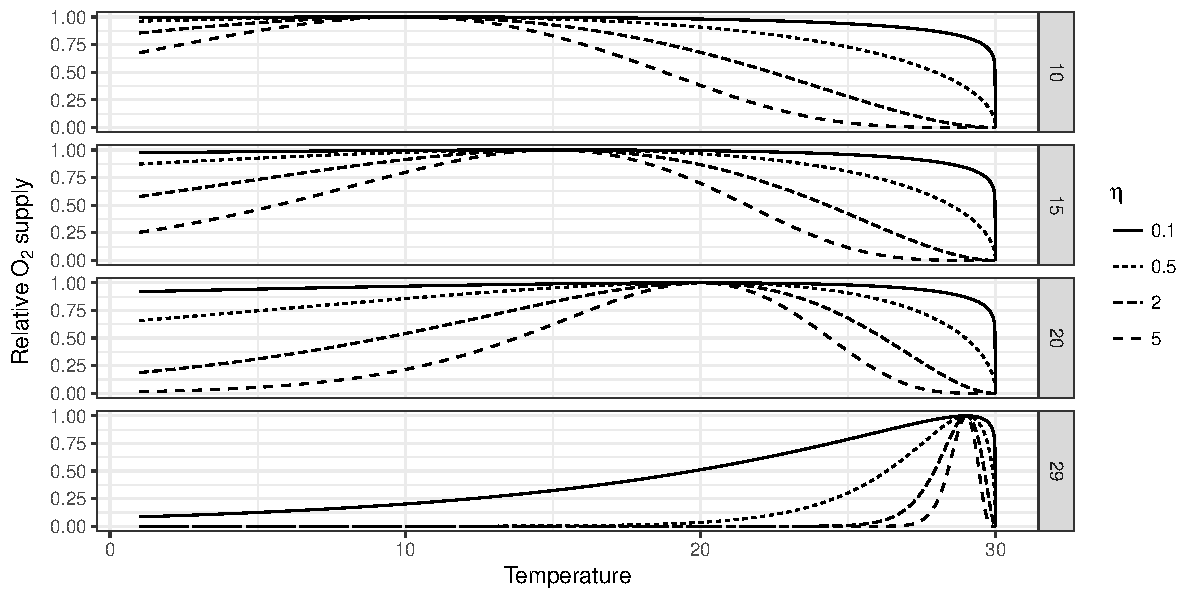
\includegraphics[width=\linewidth]{images/O2_fig-1} \caption[Maximum metabolic rate, determined by oxygen supply, as a function of temperature, for four different optimal temperatures (panels---see panel label for optimal temperature in degrees celsius), and increasing values of $\eta$]{Maximum metabolic rate, determined by oxygen supply, as a function of temperature, for four different optimal temperatures (panels---see panel label for optimal temperature in degrees celsius), and increasing values of $\eta$.}\label{fig:O2_fig}
\end{figure}




In pour model, fish will adjust their activity fraction $\tau$ to maximise fitness. We use Gilliam's rule as a fitness proxy \cite{gilliam_habitat_1987}:
\begin{equation}
  \tau^* = \text{argmax}_{\tau} \{ \frac{P(w,T)}{M(w)} \}.
\end{equation}
This optimisation represents a "short-sighted" fitness optimisation that does not account for future changes in conditions, and is appropriate for optimisation in stable environments (\cite{sainmont_effective_2015}).  Mortality scales with activity fraction and weight as $w^{q-1}$ (\cite{andersen_how_2009, hartvig_food_2011}):
\begin{equation}
  \label{eq:M}
  M(w) = (\rho+\eta\tau) w^{q-1},
\end{equation}
$\rho$ is mortality at mass $w=1$ and $\tau=0$, that is, with no activity beyond that covered by standard metabolism.  Activity is limited by available oxygen, such that the aerobic scope $P_{O_2}$ is not allowed to be negative over the time scales considered. In other words, we consider time scales that are long enough to ignore the ability of many ectotherms to go into oxygen debt, or to switch to anaerobic metabolism for limited periods of time. This means we assume that animals will adjust their foraging effort to optimise fitness given temperature and oxygen constraints. Note, that this optimal foraging assumption drives ecological responses as a consequence of physiological constraints, rather than as a direct response to temperature itself.

\subsection*{Defining performance metrics}

Performance itself is a vague concept that is often used without definition in the relevant literature, but it is only defined in the context of a particular physiological or demographic parameter, with potentially different thermal response curves (\cite{jutfelt_oxygen-and_2018}). For instance, even though growth in ectotherms is often impacted by temperature (\cite{angilletta_temperature_2004}), measured performance may depend strongly on what aspect of growth is measured --- whether it is the growth increment at a particular size, growth efficiency per unit intake, the attained asymptotic size, or parameters of a fitted growth curve. We use and compare four performance measures with broad ecological and practical implications:

\begin{itemize}

\item Growth curves predicted through ontogeny, which allow us to compare growth performance early and late in life (i.e., juvenile growth vs asymptotic size).
\item Production efficiency, here defined as available energy for both growth and reproduction, relative to the food consumption (i.e., $\frac{P(w,T)}{f(w,T)h c(T) w^q)}$.
\item The dimensionless ratio of $\frac{P}{Mw}$, which is analogous to the short-sighted fitness aproximation (Gilliam's rule) used above.
\item Fitness integrated over an individual's lifetime, defined as $R_0$ (see below).

\end{itemize}

\subsection*{Growth response}

Temperature affects growth via its effects on the energy budget and the investment of available (surplus) energy into reproduction and growth. The change in allocation to reproduction with size and age in variable environmental conditions is described by the maturation reaction norm, which is generally defined as the probability of maturing at a certain age under different growth conditions (\cite[e.g., ][]{dieckmann_probabilistic_2007}). We defined the reaction norm as the mid-point of a logistic allocation function that determines investment in reproduction as a function of age and size. 

The slope of maturation reaction norms is evolutionarily determined by the strength of the co-variation between growth and mortality for a given population in a given environment. Strongly positive co-variation leads to the relatively flat reaction norms observed for most fish populations (\cite{marty_impact_2011}). This covariation is probably the consequence of good growth conditions (e.g., from increased prey density) altering the baseline mortality $\rho$ and the risk of foraging $\eta$ (e.g., by attracting predators). We did not explicitly model these interactions here (aside from the dependence of mortality on $\tau$), but rather assumed that reaction norms evolved over regimes of relatively stable temperature and growth variation in the past. Consequently, we assumed that the evolved slope of the reaction norm is a fixed trait over the time-scales considered here for a particular species or population, and for simplicity and generality we assume a flat reaction norm (i.e., allocation to reproduction is a function of size only; fig./~\ref{fig:MRN}), although sloping reaction norms can be formulated and used in our framework (see appendix \ref{sec:MRN}). The intercept of this reaction norm was found numerically by maximising fitness ($R_0$, see below) at the reference temperature for our simulations (15\degree C), and this intercept was assumed fixed as temperatures change.

The allocation was parametrised as 
$$\phi(w^*) = 1/(1+\exp(-cw^*))$$,
where $w^*$ is the intercept of the reaction norm, and $c$ determines how rapidly energy allocation shifts from somatic growth to reproduction. 

As growth is also fundamentally driven by resource availability, we contrast the growth response to temperature at the baseline level (Table \ref{tab:parameters}), with a 1/3 reduction and increase in available resources.

\subsection*{Fitness consequences}

Fitness consequences for particular life-history strategies (trait combinations, see below) at different temperatures can be investigated if one considers the time-scales in the model to be short relative to evolutionary time-scales (i.e., if the model represents ecological time-scales). On these time-scales, we assume that adaptive responses are negligible. We investigate over-all fitness with respect to temperature by calculating $R_0$ for a given maturation-reaction norm and trait parameters - we thus do not consider evolutionary consequences of changes in fitness here. $R_0$ was calculated as 

$$R_0(T) = \int_0^\infty \phi(w(t),w^*)P(w(t),T)S_{0 \rightarrow t}(T) \text{d}t, \text{, where}$$
$$S_{0 \rightarrow t}(T) = \int_0^t \exp(-M(w(t),T))\text{d}t$$








\begin{figure}

{\centering \includegraphics[width=\maxwidth]{images/scenarios-1} 

}

\caption[Available energy $P$ (Blue solid line), efficiency (green dashed line), and the ratio of $P$ to $M$ (orange dotted line) are impacted as a function of changing activity at constant temperature ($T=15$\degree C) for a growing fish ($L_{\infty}\sim 30$cm) at 10cm length (10g)]{Available energy $P$ (Blue solid line), efficiency (green dashed line), and the ratio of $P$ to $M$ (orange dotted line) are impacted as a function of changing activity at constant temperature ($T=15$\degree C) for a growing fish ($L_{\infty}\sim 30$cm) at 10cm length (10g). Responses are shown for slow- (a) and fast strategy (b). All rates are plotted relative to their maximum for each trait scenario, the optimal activity level $\tau^*$ is indicated by the dotted vertical line.}\label{fig:scenarios}
\end{figure}



\subsection*{Trait based scenarios}

To ensure a level of generality, we explored ecological impacts of optimised behaviour at different temperatures in a trait-based context. Specifically, we aimed to contrast species along a gradient of life-history that, at the one end, maximises production (energy acquisition; henceforth called the fast strategy, indicated by a subscript $f$) at the cost of increased metabolism and mortality, and at the opposing end minimises mortality and metabolic costs at the expense of production (henceforth slow strategy, indicated by a subcript $s$). This axis leads to an approximately constant ratio of production to mortality, and corresponds to a line of equal size in the life-history space proposed by \citeauthor{charnov_evolutionary_2013} (\citeyear{charnov_evolutionary_2013}). In other words, this axis contrasts species of similar size (here $L_{\infty}\sim 30$cm or $w_{\infty}\sim 270$g) with defensive/sluggish versus active life-histories.

To implement this axis, we used the result that species with a more
active, production oriented life-history (e.g., predatory pelagic
fish) have a higher standard metabolism and lower weight scaling of
metabolic costs
(\cite{priede_metabolic_1985,killen_intraspecific_2010}). We assumed
that higher standard metabolism is due to increased digestive capacity
(i.e., is used for gut maintenance), though high muscle mass and a
larger heart will also contribute to higher standard metabolism in
active species (\cite{priede_metabolic_1985}). In practice, we assumed
that approximately 50\% of the standard metabolic cost is due to gut
maintenance, such that a doubling of the maximum ingestion leads to a
50\% increase in standard metabolic cost. We further assumed that such active species have a less effective refuge from predators and therefore have a higher constant mortality, but lower mortality related to activity (i.e., $M_{s}(w) = (0.1+6\tau) w^{q-1}$ and $M_{f}(w) = (1+\tau) w^{q-1}$). Exact parameter values for these trait scenarios are given in Table \ref{tab:parameters}. Together, these assumed trait differences lead to very different ecological and bio-energetic responses of slow- and fast strategists (fig./~\ref{fig:scenarios}), with $\tau_{\text{opt}}$ found at lower activity levels for slow-strategists, as high activity induces exceedingly high mortality and decreasing energy efficiency (i.e., available energy relative to food intake) at high activity levels. A slower increase in available energy and M with $\tau$ for fast strategists leads to a higher $\tau_{\text{opt}}$.



We further contrasted species with oxygen limitation at high temperatures (i.e., species with a uni-modal metabolic scope) with species that do not experience oxygen limitation at high temperatures (at least not up to a lethal temperature, where death may be induced by sudden failure to deliver oxygen to vital organs, or failure of bio-chemical pathways at high temperature \cite{salin_inadequate_2016,iftikar_mitochondria_2013}). In practice, this was achieved as described above by setting the maximum oxygen delivery close to the lethal temperature (fig./~\ref{fig:O2_fig}). Note that, although we assume here that limitations over the temperature range are due to oxygen availibility, other limiting mechanisms, such as the respiratory control ratio (\cite{salin_inadequate_2016,iftikar_mitochondria_2013}) may determine upper limits to activity over some or all of a species temperature range. However the over-all mechanism would be the same to the one assumed here, with different untis (e.g., ATP instead of $O_2$).

\begin{table}
\caption{Parameters of the constrained activity model for two scenarios: slow strategy and fast strategy species. For parameters with dual values (i.e., x/y), the former reflects species with a domed maximum oxygen supply (MOS) with respect to temperature, whereas the latter corresponds to species with a continuously increasing MOS. Values in brackets for $\gamma$ are alternative resource availability scenarios.}
\label{tab:parameters}
\begin{tabular}{llcc}
 \multirow{2}{*}{Description} &  \multirow{2}{*}{Symbol (unit)} & \multicolumn{2}{r}{Value} \\
 \cmidrule{3-4}
 & & slow strategy  & fast strategy \\

\hline
\addlinespace
\multicolumn{4}{c}{\textbf{Biomass Metabolism}} \\
Specific dynamic action & $\beta$ & \multicolumn{2}{c}{0.15} \\
Egestion and excretion & $\phi$ & \multicolumn{2}{c}{0.25}  \\
Coeff. for std.~metabolism  & $k$ (g$^{1-n}\cdot$y$^{-1}$)  & 1 &  1.5 \\
Coeff. for act.~metabolism  & $k$ (g$ \cdot$y$^{-1}$)  & 4 &  2 \\
Exponent for std.~metabolism & $n$ & 0.88 & 0.75  \\

\addlinespace
\multicolumn{4}{c}{\textbf{Feeding ecology}}\\
Coeff. for Encountered food & $\gamma\Theta$ (g$^{1-p} \cdot$y$^{-1}$)& \multicolumn{2}{c}{60 (40/80)} \\
Exponent for clearance rate $\gamma$ & $p$ & \multicolumn{2}{c}{0.8}  \\
Coeff. for Maximum consumption rate & $h$ (g$^{1-q}\cdot$y$^{-1}$) & 30 & 60  \\
Exponent for max.~consumption $h$ & $q$ & \multicolumn{2}{c}{0.8} \\
Coeff. for constant mortality & $M$ (g$\cdot$y$^{-1}$) & 0.1  & 1  \\
Coeff. for activity related mortality & $\rho$(y$^{-1}$) & 6 & 1\\
Exponent for mortality & $\nu$ & \multicolumn{2}{c}{0.2} \\

\addlinespace
\multicolumn{4}{c}{\textbf{Temperature}}\\
Reference temperature  & $T_{\text{ref}}$ (°C)& \multicolumn{2}{c}{15} \\
Activation energy & $E_a$ & \multicolumn{2}{c}{0.52} \\
Temperature at maximum MOS & $T_{\text{max}}$ & \multicolumn{2}{c}{20/25}\\
Temperature range & $T^-_{\text{lethal}}$--$T^+_{\text{lethal}}$ & \multicolumn{2}{c}{5--26} \\

\addlinespace
\multicolumn{4}{c}{\textbf{Reaction norm}}\\

Slope &  & \multicolumn{2}{c}{0}\\
Reaction & $c$ & \multicolumn{2}{c}{0.5} \\

\addlinespace
\multicolumn{4}{c}{\textbf{Oxygen budget}} \\
Critical $O_2$ & $P_{\text{crit}}$ (mg$\cdot$L$^{-1}$) & \multicolumn{2}{c}{2}\\
Dissolved $O_2$ at $0.5\times f_{\text{max}}(O_2)$  & $P_{50}$ (mg$\cdot$L$^{-1}$) & \multicolumn{2}{c}{4} \\
Doming for $O_2$ supply & $\eta$ & \multicolumn{2}{c}{3/0.1}\\
Level of $O_2$ supply  & $\zeta$ (g$\cdot$y$^{-1}$) &  0.5 & 1\\


\hline
\end{tabular}
\end{table}




\section*{Results}

Increasing metabolic demands with temperature lead species to adjust activity levels in order to optimise energy gains relative to mortality risk (fig./~\ref{fig:activity}). This adjustment is especially pronounced in slow strategy species, for which the over-all activity level is markedly lower and which show a consistent increase in activity over-all sizes for the simulated life-history (fig./~\ref{fig:size-act}). A similar increase in activity is observed for small fast strategy individuals (e.g., post-larval) for which even initial activity levels are very high (fig./~\ref{fig:size-act}). For these individuals, the increasing activity and metabolic demands lead to an active metabolic rate that is close to their MMR. For all other sizes across the two trait scenarios, oxygen is only limiting to activity at the extremes of the simulated temperature range (fig./~\ref{fig:activity}), and only for species with a dome-shaped MOS with respect to temperature. For species with a rising MOS with temperature, oxygen is not limiting (fig./~\ref{fig:activity-rising}). However, larger fast strategy individuals are predicted to show a slightly dome-shaped adjustment in activity levels at intermediate sizes, and a slightly decreasing activity level in response to temperature at large sizes, despite available aerobic scope for activity. This adjsutment is a function of metabolic activity costs assumed here - at smaller metabolic costs per activity, activity adjustment are strictly increasing (fig./~\ref{fig:size-act_low}).


\begin{figure}
\centering

\includegraphics[width=\maxwidth]{images/activity-1} 

\caption{Optimum (red long-dashed), maximum (green short-dashed) and realised (blue solid lines) activity levels (left column [a,c]) at increasing temperatures for a 10g fish with a dome-shaped MOS with increasing temperature (maximum at 20\degree C), with corresponding oxygen demand (right column [b,d]); maximum oxygen supply (MOS; green short-dashed), standard metabolism (red long-dashed) and realised (active; blue solid lines) metabolic demand, as well as metabolic scope (orange long-dashed) at activity level $\tau$, for slow strategy (slow life history; a \& b) and fast strategy (fast life-history; c \& d).}
\label{fig:activity}
\end{figure}



\begin{figure}

{\centering \includegraphics[width=\maxwidth]{images/size-act-1} 

}

\caption[Optimum (red long-dashed), maximum (green short-dashed) and realised (blue solid lines) activity levels (left column) at increasing temperatures through ontogeny for a for fish with a $L_{\infty}\sim 30$cm at 1.25g (5cm]{Optimum (red long-dashed), maximum (green short-dashed) and realised (blue solid lines) activity levels (left column) at increasing temperatures through ontogeny for a for fish with a $L_{\infty}\sim 30$cm at 1.25g (5cm; a--b); 10g (10cm; c--d) and 80g (20cm; e--f), for slow strategy (slow life history; left column [a,c,e]) and fast strategy (fast life-history; right column [b,d,f]) species with a dome-shaped maximum metabolic rate with respect to temperature.}\label{fig:size-act}
\end{figure}



Temperature and metabolic demand-driven adjustments to the activity level lead to substantial changes in performance related metrics in both trait scenarios (fig./~\ref{fig:feeding}). For slow strategy species, the increases in activity levels lead to relatively stable feeding levels, but a substantial increase in mortality coupled with a slow increase in available energy leads to an over-all decline in the ratio of $P$ to $M$. Available energy shows a dome-shaped response to temperature in slow strategists, and is maximised at relatively high temperatures. However, it is limited by oxygen availability only at high temperatures in species with a dome-shaped MOS. Production efficiency follows a near opposite trend due to the relatively flat response in the feeding level $f$, but temperature driven increases in maximum consumption.

For fast strategists, the relatively modest response in activity levels at all but the smallest sizes leads to a decline in feeding levels, which causes a largely dome-shaped response of available energy and growth efficiency to warmer temperatures (fig./~\ref{fig:feeding}). Again, production efficiency peaks at relatively low temperatures, but in this scenario available energy $P$ peaks at much lower temperatures. Given the relatively flat mortality levels, the ratio of $P/M$ largely follows the trend in $P$. 

\begin{figure}

{\centering \includegraphics[width=\maxwidth]{images/feeding-1} 

}

\caption[Feeding level (blue solid line), available energy $P$ (green long-dashed), efficiency (orange dotted), mortality (red dotted-dashed) and the ratio of $P$ to $M$ (yellow solid) are impacted by changing activity and the metabolic response to temperature for a growing fish ($L_{\infty}\sim 30$cm) at 10cm length (10g)]{Feeding level (blue solid line), available energy $P$ (green long-dashed), efficiency (orange dotted), mortality (red dotted-dashed) and the ratio of $P$ to $M$ (yellow solid) are impacted by changing activity and the metabolic response to temperature for a growing fish ($L_{\infty}\sim 30$cm) at 10cm length (10g). Responses are shown for slow  and fast strategy (a and b, respectively), for species with and without oxygen limitation (left and right columns, respectively). Energy, mortality and fitness are plotted relative to their maximum over all temperatures.}\label{fig:feeding}
\end{figure}



Simulated growth curves illustrate the ontogenetic consequences of increasing temperatures (fig./~\ref{fig:norms}). For both trait scenarios, fastest growth occurred at relatively high temperatures, with declining growth for oxygen limited species at the highest temperatures (fig./~\ref{fig:norms_O2}). This can be explained by ontogenetic shifts in temperature optima for growth (fig./~\ref{fig:size-rates}): for small individuals, available energy and growth consistently peak at high temperatures, but this peak rapidly moves to lower temperatures as individuals in either trait-scenario grow. For large individuals, growth is optimised at relatively low temperatures, leading to larger asymptotic size at lower temperatures. 

Resource availability strongly modulates this growth response to temperature: low resource availability leads to strong differences in asymptotic size, whereas high food availability leads to fast growth and larger asymptotic length at high temperatures (figs./~\ref{fig:norms},\ref{fig:infs}). In addition, in very resource poor conditions, individuals may not grow to reproductive size in our scenario of a flat MRN. Over-all growth responses to temperature are not strongly affected by the assumed slope of the MRN (figs. \ref{fig:norms_neg},\ref{fig:norms_pos}), although a negatively sloped MRN does ensure maturation in low resource environments.




\begin{figure}

{\centering \includegraphics[width=\maxwidth]{images/norms-1} 

}

\caption[On ecological time-scales, increasing temperature (purple to yellow growth curves) modifies growth, and maturation age changes according to the reaction norm (black dots at 50\% allocation to reproduction), whereas asymptotic size is affected by changes in absolute energy available for growth]{On ecological time-scales, increasing temperature (purple to yellow growth curves) modifies growth, and maturation age changes according to the reaction norm (black dots at 50\% allocation to reproduction), whereas asymptotic size is affected by changes in absolute energy available for growth. Growth curves are shown for slow- (left column [a,c,e]) and fast strategists (right column [b,d,f]), at increasing food availibility from top (a/b) to bottom (e/f). Baseline resource availibility assumed in all other simulations is that shown in panels c and d.}\label{fig:norms}
\end{figure}



\begin{figure}

{\centering \includegraphics[width=\maxwidth]{images/infs-1} 

}

\caption[Interactive effects of food availibility and temperature of the asymptotic size ($L_{\infty}$), with increasing linewidth showing increasing prey availibility for a) slow and b) fast life-history species]{Interactive effects of food availibility and temperature of the asymptotic size ($L_{\infty}$), with increasing linewidth showing increasing prey availibility for a) slow and b) fast life-history species.}\label{fig:infs}
\end{figure}



Over-all fitness consequences mirror trends in the ratio of $P/M$ (fig./~\ref{fig:fit}a), which can be seen as a short sighted approximation to over-all fitness optimisation (\cite{sainmont_effective_2015}). With increasing temperatures, fitness declines at our basic parameter settings, in opposition to growth and aerobic scope. At low temperatures, fitness is limited by aerobic scope, with the magnitude determined by the extend of doming in aerobic scope. Note that this limitation through the aerobic scope appears at higher temperatures than apparent from fig./~\ref{fig:activity}, reflecting stronger limitation of oxygen on growth during early life (fig./~\ref{fig:size-rates}). Fitness trends with temperature are strongly dependent on metabolic costs of activity (fig./~\ref{fig:fit}b), and changing the activity cost to lower values attenuates the decline in fitness with temperature for slow strategy species, and moves the fitness optimum to higher temperatures for fast strategy species. Similarly, increased food availibility leads to changes in fitness optima, with higher optimum temperatures, especially for fast strategists, and a slower decline of fitness with temperature.



\begin{figure}

{\centering \includegraphics[width=\maxwidth]{images/fit-1} 

}

\caption[Fitness ($R_0$), relative to maximum fitness within (a and b) oxygen limited (blue) and non-oxygen limited (teal) for slow- (a) and fast strategy (b) species at the assumed maturation-raction norm and base parameters, and (c and d) changes in relative fitness with respect to temperature resulting from decreasing levels of activity cost symbolised by decreasing linewidth, and (e and f) changes in relative fitness with respect to temperature as a function of increasing food availability (increasing linewidth)]{Fitness ($R_0$), relative to maximum fitness within (a and b) oxygen limited (blue) and non-oxygen limited (teal) for slow- (a) and fast strategy (b) species at the assumed maturation-raction norm and base parameters, and (c and d) changes in relative fitness with respect to temperature resulting from decreasing levels of activity cost symbolised by decreasing linewidth, and (e and f) changes in relative fitness with respect to temperature as a function of increasing food availability (increasing linewidth)}\label{fig:fit}
\end{figure}




\section*{Discussion}

In this study, we attempt to provide a general mechanistic basis for exploring thermal sensitivities of ectotherm organisms. Much of the recent debate about the validity of projected climate change impact on ectotherms, and fish in particular, has resolved about the validity of particular concepts, such as the OCLTT and projections based on the gill-oxygen limitation theory (\cite{pauly_sound_2017,lefevre_modelling_2017}). We attempted to go beyond this debate by developing a model that allows for general insights about the temperature response in ectotherms, while being specific enough to mechanistically articulate aspects of physiology and ecology that are fundamental to organism response to temperature. The general model and its parameter values are also easily adjusted to reflect particular organisms or theories. 

It has been argued that the OCLTT as a concept provides a basis to explain observed responses to climate change on the basis of oxygen limitation via the aerobic scope (\cite{portner_physiology_2008,portner_oxygen-and_2010}), and simple oxygen budgets have been used to predict metabolic constraints on organismal activity due to warming ocean temperatures (\cite{deutsch_climate_2015}). As a conceptual framework, however, the OCLTT is subject not only to semantic dispute but also criticism of its core concept of oxygen limitation (\cite{jutfelt_oxygen-and_2018,lefevre_are_2016}).

Our quantitative thermal impact model generalises existing eco-physiological models for particular species and stocks (\cite{hufnagl_physiological_2011, holt_climate_2014,holt_climate_2015}), and allows to develop a more nuanced understanding of interactions between temperature, oxygen limitation and ecology for species with varying traits. In line with the conceptual framework of Fry's aerobic scope and the OCLTT, our model suggests that oxygen limitation can be a potentially important ecological driver, especially at extreme temperatures for species with declining MOSs in such temperature regimes. At the onset of this limitation, ecological parameters change drastically, and growth, mortality are strongly impacted. This limitation closely mimics limitations seen in wild fish (\cite{myrick_temperature_2000}), and is in line with observations that fish often seek specific water temperatures to optimise metabolic function (\cite[e.g., ][]{armstrong_diel_2013,claireaux_physiology_1995}). Fitness, however, appears to be limited through the metabolic scope primarily via limitations at temperature extremes and impact on particular life-history stages. For instance, oxygen limitation is a more severe constraint for small individuals (fig./~\ref{fig:size-rates}), and thereby can limit growth performance early in life, impacting over-all fitness. Furthermore, changes in environmental oxygen supply, if beyond an organisms ability to compensate via passive or active compensation mechanisms, will induce an over-all lower aerobic scope and lead to an earlier onset of oxygen limitation, but such scenarios do not change the qualitative predictions from our model.

Variation in performance metrics away from temperature extremes are primarily affected by the interaction of temperature driven metabolic demands with optimal feeding behaviour. Predictions from our model, in line with metabolic experiments and species specific physiological predictions (\cite[e.g., ][]{holt_climate_2014}), suggest that routine activity, including normal swimming behaviour, feeding, and digestion usually lead to routine metabolic rates that are well below the MOS, even in fish with high metabolism (\cite{lucas_utilization_1992,priede_metabolic_1985}). Strenuous swimming activity, for example, usually only makes up a small proportion of the standard energy budget in fish (\cite{priede_natural_1977,priede_metabolic_1985}). Furthermore, as a limit for long-term performance, the MOS does not usually impose a limitation on short term energy demands, as fish can incur oxygen debt during swimming bursts during which the MOS is exceeded (\cite{brett_metabolic_1972,priede_metabolic_1985}). A logical conclusion is that the metabolic scope is only limiting to performance at extreme temperatures where MOS is low due to impaired oxygen delivery.

In many species, both the aerobic scope and growth peak at relatively high temperatures within the potential thermal range, yet species are often found at temperatures lower than these optima (\cite{magnuson_thermal_1997, claireaux_influence_2000}). Previous explanations of this niche-occupation paradox involved environmental factors that narrow the thermal niche or behaviour that optimises thermal performance across available habitats (\cite{claireaux_influence_2000, magnuson_thermal_1997}). In nearly all our simulation scenarios, fitness is predicted to decline with increasing temperature. This decline with temperature leads to a parsimonious explanation for the relationship between growth performance and fitness at varying temperatures.s

Resource availability imposes a strong environmental constraint on organisms, with all aspects from optimal activity levels, mortality and available energy for growth ultimately influenced by available prey. Changes in prey availability thus influence individual temperature response directly via available energy, and indirectly, through altered energetic requirements to procure food and changes in mortality due to changes in the optimal activity level. In low-food environments, changing energetic demands with temperature are not easily adjusted for, and any adjustment demands higher energetic costs and mortality risk. This environment-driven change in costs of temperature adjustments leads to the strong modulation of the growth response, as well as changing gradients in fitness with temperature in these environments. In particular, in low-food environments, asymptotic size is strongly reduced at high temperatures, whereas this is not necessarily the case in high-food environments. Increased growth and mortality changes in such environments then combine to produce a more strongly domed fitness curve than in environments where food supply is not limiting.

Our model prediction of declining fitness with temperature is
particularly sensitive to activity costs, with low activity costs
leading to increased fitness at warmer temperatures. Our
base-parametrisation is based on the assumption that activity cost $k_a$ reflects the cost of maximal activity (i.e., cost of
$\tau=1$), and has the same pay-off for all life-histories. This approximation may not
reflect actual activity cost as swimming at MMR in fast predatory fish
is far more efficient than swimming of sluggish fish, such as flatfish
(\cite{priede_metabolic_1985}). Such an efficiency gain may occur as a result of more efficient form or physiology, or simply by reduced drag at large size (e.g., whale-sharks), and may be a key requirement to the viability of active pelagic predatory fish in tropical waters.

That fish behave optimally to maximise food acquisition relative to mortality risk and energetic requirements is a standard hypothesis and assumption in ecological models (\cite{gilliam_habitat_1987,sainmont_effective_2015,priede_natural_1977, claireaux_influence_2000,hufnagl_physiological_2011}). Indeed, heightened mortality risk may be a key driver of fish spending very little time \emph{in vivo} at metabolic regimes that approach the MOS (\cite{priede_natural_1977}), an observation that is in line with predictions from our model, especially for the slow (slow strategy) life-history. Our scenarios were parametrised to allow for excess metabolic scope beyond maximum foraging activity (i.e., $\tau=1$). This assumption is in line with observations that the aerobic scope often exceeds energetic requirements from swimming alone, and is adapted to provide oxygen for digestion (SDA), the oxygen demand of which can be as high or higher than that of locomotion alone (\cite{priede_metabolic_1985}).

Optimal activity is predicted to increase with temperature in nearly all cases, but it is sensitive to the cost of activity - at higher cost relative to the potential pay-off, activity may even decline at high temeprature. Predictions of increased activity are supported by many observations in experimental and field conditions for both larval and adult fish (\cite{sswat_growth_2018,brown_feeding_1989,claireaux_physiology_1995, biro_mechanisms_2007}). This increase of activity often occurs despite increased mortality (\cite[e.g., ][]{sswat_growth_2018, biro_mechanisms_2007}), and serves the necessity to offset increased metabolic expenses. Only large individuals of the simulated fast strategy species will optimally decrease activity as a result of increased temperature. In this case, additional activity will lead to comparatively small gains from feeding relative to the cost of activity and SDA, owing to the non-linearity of the functional response.

Taken together, the physiological processes and optimisation described in our model provide a mechanistic underpinning for observations about changes of ecological rates, such as
increasing or dome-shaped consumption or attack-rates with temperature
(\cite{biro_mechanisms_2007,englund_temperature_2011,rall_universal_2012}). Depending on the
strength of oxygen limitation and the development of the optimal
activity level over the range of temperatures considered, attack rates
and feeding rates may appear to be steadily increasing via increased
optimal activity, or dome-shaped from oxygen limitation or dome-shaped
optimal activity. Thus, rather than assuming \emph{ad hoc} changes in ecological rates in response to temperature that may not be transferable between species and traits, the change in these rates may be mechanistically described in terms of optimal ecological adjustments to physiological constraints.

Similarly, our model provides a mechanistic basis for the temperature-size rule in ectotherms (\cite{atkinson_temperature_1994}), without needing to evoke direct changes in ecological rates with temperature. The physiological basis leads to heterogeneous predictions about growth trajectories over ranges of temperature, with various degrees of nesting (i.e., non-crossing) and crossing of growth trajectories possible depending on ecological conditions (e.g., food availability) and physiological traits (figs \ref{fig:norms}, \ref{fig:norms_O2}). Due to its reliance on physiological traits and their interaction with ecological variables, our model provides a multi-variate framework to predict heterogeneous temperature impacts on size and growth (\cite{angilletta_temperature_2004}).

In order to provide a general framework, our model setup is deliberatly minimalist, and probably under-parametrised to reflect ecological and life-history aspects of particular species, such as migrations, social behaviour or seasonal energy requirements. As such, this framework provides a null model to assess the diversity of possible responses in fish, and other ectotherms, to temperature in a highly simplified system. Nevertheless, it provides a starting point from which to explore the importance of costs and benefits of particular life-histories and thermal adaptations. For instance, a recent species-specific eco-physiological model for cod (\emph{Gadus morhua}) that includes similar physiological constraints to our model predicted relatively high fitness at high temperatures (\cite{holt_climate_2014,holt_climate_2015}). Although this difference is potentially due to the different activity cost coefficients, foraging assumptions and species specific parametrisations in their model, differences may also be due to key assumptions about optimal reproduction: the model of  \textcite{holt_climate_2014} assumed that reproductive investment is instantaneously optimised in a changing climate, pointing to the possibility that adaptation of reproductive patterns could offset potential fitness declines with increasing temperatures.

\section*{Conclusions}

The importance of the interaction between ecology, bio-energetics and oxygen limitations in deriving realistic predictions about temperature impacts on ecological rates and fitness calls into question predictions for climate change impacts based on simple models of growth alone (\cite{cheung_shrinking_2013, pauly_sound_2017}). We suggest that the general trait-based approach presented here provides a parsimonious compromise between simplistic approximations that may provide misleading predictions about future ecosystems (\cite{brander_overconfidence_2013, lefevre_models_2017}), and more complex eco-physiological models such as dynamic energy budget models (\cite[e.g., ][]{guiet_effects_2016}) and species specific eco-physiology models (\cite{hufnagl_physiological_2011, holt_climate_2014,holt_climate_2015}). In addition, our model provides a more explicit, physiology-based mechanistic model to derive general predictions about temperature effects on ectotherms than previous general frameworks such as the OCLTT. Predictions from the OCLTT are both contributing to patterns in fitness and ecological rates shown here, but are also only part of the picture, and we suggest that future improvements of predictive frameworks should center on model critisism and improvements, and leave behind semantic discussions about conceptual constructs that are difficult to explicitly link to data.

% \section*{Acknowledgments}
% 
% The authors would like to thank members of the DTU Centre for Ocean Life modeling group for stimulating discussions over the course of the development of the ideas in this paper. PN was supported by a Marsden fast-start grant by the Royal Society Te Apārangi of New Zealand. KHA was supported by the Centre for Ocean Life, a VKR Centre of Excellence funded by the Villum Foundation.

\newpage{}

\titleformat{\section}{\normalfont\bfseries\sffamily}{APPENDIX \thesection:}{1em}{}
\renewcommand{\theequation}{\thesection-\arabic{equation}}
\renewcommand{\thetable}{\thesection-\arabic{table}}
\renewcommand{\thefigure}{\thesection-\arabic{figure}}
\setcounter{figure}{0}  % reset counter 
\setcounter{table}{0}  % reset counter 
\setcounter{equation}{0}  % reset counter 

\section*{Maturation-reaction norm}
\label{sec:MRN}

A flat maturation reaction norm (MRN) leads to a logistic allocation to reproduction that is only dependent on size and independent of age (fig./~\ref{fig:MRN}).

\begin{figure}

{\centering \includegraphics[width=\maxwidth]{images/MRN-1} 

}

\caption[Proportion of energy allocated to reproduction, as a function of age (a) and size (b)]{Proportion of energy allocated to reproduction, as a function of age (a) and size (b). With a flat maturation-reaction norm, maturation is independent of age, and only size-dependent.}\label{fig:MRN}
\end{figure}



To express a MRN that varies as a function of age, we can reparametrise the MRN as:
$$\phi(z) = 1/(1+\exp(-(c z))) \text{, where }$$
$$z(t, w_t) = (w_t-w^*)\times \text{cos}(\text{atan}(b))-t\times \text{sin}(\text{atan}(b))$$  
rotates the coordinate system about the slope $b$ of the reaction norm, $t$ is the age, $w$ is the mass, $w^*$ is the intercept of the reaction norm, and $c$ determines how rapidly energy allocation shifts from somatic growth to reproduction. 

\section*{Supplementary results}

\begin{figure}
\centering

\includegraphics[width=\maxwidth]{images/activitys-1} 

\caption{Optimum (red long-dashed), maximum (green short-dashed) and realised (blue solid lines) activity levels (left column [a,c]) at increasing temperatures for a 10g fish with a continuously increasing MOS with increasing temperature, with corresponding oxygen demand (right column [b,d]); maximum oxygen supply (MOS; green short-dashed), standard metabolism (red long-dashed) and realised (active; blue solid lines) metabolic demand, as well as metabolic scope (orange long-dashed) at activity level $\tau$, for slow strategy (slow life history; aandb) and fast strategy (fast life-history; c, d).}
\label{fig:activity-rising}
\end{figure}

\begin{figure}

{\centering \includegraphics[width=\maxwidth]{images/size-act_low-1} 

}

\caption[Optimum (red long-dashed), maximum (green short-dashed) and realised (blue solid lines) activity levels at increasing temperatures through ontogeny for a for fish nearly grown fish of 80g (20cm]{Optimum (red long-dashed), maximum (green short-dashed) and realised (blue solid lines) activity levels at increasing temperatures through ontogeny for a for fish nearly grown fish of 80g (20cm; e--f), for a fast strategy (fast life-history) species with a dome-shaped maximum metabolic rate with respect to temperature. }\label{fig:size-act_low}
\end{figure}



\begin{figure}

{\centering \includegraphics[width=\maxwidth]{images/size-rates-1} 

}

\caption[Feeding level (blue solid line), available energy $P$ (green long-dashed), efficiency (orange dotted), mortality (red dotted-dashed) and the ratio of $P$ to $M$ (yellow solid) are impacted by changing activity and the metabolic response to temperature for growing fish ($L_{\infty}\sim 30$cm) of 1.25g (5cm]{Feeding level (blue solid line), available energy $P$ (green long-dashed), efficiency (orange dotted), mortality (red dotted-dashed) and the ratio of $P$ to $M$ (yellow solid) are impacted by changing activity and the metabolic response to temperature for growing fish ($L_{\infty}\sim 30$cm) of 1.25g (5cm; a--b); 10g (10cm; c--d) and 80g (20cm; e--f ), for slow strategy (slow life history; left column [a,c,e]) and fast strategy (fast life-history; right column [b,d,f]) species with a dome-shaped maximum metabolic rate with respect to temperature. Energy, mortality and fitness are plotted relative to their maximum over all temperatures.}\label{fig:size-rates}
\end{figure}




\begin{figure}
\centering


{\centering \includegraphics[width=\maxwidth]{images/norms_O2-1} 

}



\caption{Contrasting growth responses at baseline resource availability for species with dome-shaped MOS (top row [a,b]) and increasing MOS with temperature (bottom row [c,d]). Growth curves are shown for slow- (left column [a,c]) and fast strategists (right column [b,d]). Increasing temperature (purple to yellow growth curves) modifies growth, and maturation age changes according to the reaction norm (black dots at 50\% allocation to reproduction), whereas asymptotic size is affected by changes in absolute energy available for growth.}
\label{fig:norms_O2}
\end{figure}





\begin{figure}

{\centering \includegraphics[width=\maxwidth]{images/norms_neg-1} 

}

\caption[On ecological time-scales, increasing temperature (purple to yellow growth curves) modifies growth, and maturation age changes according to the negative reaction norm (black dots at 50\% allocation to reproduction), whereas asymptotic size is affected by changes in absolute energy available for growth]{On ecological time-scales, increasing temperature (purple to yellow growth curves) modifies growth, and maturation age changes according to the negative reaction norm (black dots at 50\% allocation to reproduction), whereas asymptotic size is affected by changes in absolute energy available for growth. Growth curves are shown for slow- (left column [a,c,e]) and fast strategists (right column [b,d,f]), at increasing food availibility from top (a/b) to bottom (e/f). Baseline resource availibility assumed in all other simulations is that shown in panels c and d.}\label{fig:norms_neg}
\end{figure}






\begin{figure}

{\centering \includegraphics[width=\maxwidth]{images/norms_pos-1} 

}

\caption[On ecological time-scales, increasing temperature (purple to yellow growth curves) modifies growth, and maturation age changes according to the positive reaction norm (black dots at 50\% allocation to reproduction), whereas asymptotic size is affected by changes in absolute energy available for growth]{On ecological time-scales, increasing temperature (purple to yellow growth curves) modifies growth, and maturation age changes according to the positive reaction norm (black dots at 50\% allocation to reproduction), whereas asymptotic size is affected by changes in absolute energy available for growth. Growth curves are shown for slow- (left column [a,c,e]) and fast strategists (right column [b,d,f]), at increasing food availibility from top (a/b) to bottom (e/f). Baseline resource availibility assumed in all other simulations is that shown in panels c and d.}\label{fig:norms_pos}
\end{figure}




\end{document}
